% Copyright (c) 2017-2020 Matematyka dla Ciekawych Świata (http://ciekawi.icm.edu.pl/)
% Copyright (c) 2017-2020 Robert Ryszard Paciorek <rrp@opcode.eu.org>
% 
% MIT License
% 
% Permission is hereby granted, free of charge, to any person obtaining a copy
% of this software and associated documentation files (the "Software"), to deal
% in the Software without restriction, including without limitation the rights
% to use, copy, modify, merge, publish, distribute, sublicense, and/or sell
% copies of the Software, and to permit persons to whom the Software is
% furnished to do so, subject to the following conditions:
% 
% The above copyright notice and this permission notice shall be included in all
% copies or substantial portions of the Software.
% 
% THE SOFTWARE IS PROVIDED "AS IS", WITHOUT WARRANTY OF ANY KIND, EXPRESS OR
% IMPLIED, INCLUDING BUT NOT LIMITED TO THE WARRANTIES OF MERCHANTABILITY,
% FITNESS FOR A PARTICULAR PURPOSE AND NONINFRINGEMENT. IN NO EVENT SHALL THE
% AUTHORS OR COPYRIGHT HOLDERS BE LIABLE FOR ANY CLAIM, DAMAGES OR OTHER
% LIABILITY, WHETHER IN AN ACTION OF CONTRACT, TORT OR OTHERWISE, ARISING FROM,
% OUT OF OR IN CONNECTION WITH THE SOFTWARE OR THE USE OR OTHER DEALINGS IN THE
% SOFTWARE.

\subsection{Warsztat – płytka stykowa, przewody i śrubokręt}

Kolejnymi rzeczami w które warto się zaopatrzyć są elementy umożliwiają łatwe budowanie układów prototypowych:
\begin{itemize}
	\item płytka prototypowa stykowa (jedna lub dwie)
	\item przewody męsko-męskie (około 30sztuk)
	\item przewody męsko-żeńskie (około 10sztuk)
	\item przewody żeńskie-żeńskie (opcjonalnie, około 10sztuk)
	\item przewody pin męski - krokodylek lub krokodylek-krokodylek (około 5sztuk)
	\item śrubokręt mały płaski
\end{itemize}

\vspace{12pt}
\hspace{\stretch{2}}
	\parbox[c]{0.45\textwidth}{
		\includegraphics[height=5.3cm]{warsztat_elektroniczny/płytka_i_przewody}\footnotesize
		\\na górze od lewej: przewód męsko-męski (czerwony), żeńsko-żeński (czarny) i męsko-żeński (żółty);
		\\poniżej przykładowa płytka stykowa
	}
\hspace{\stretch{1}}
	\parbox[c]{0.45\textwidth}{
		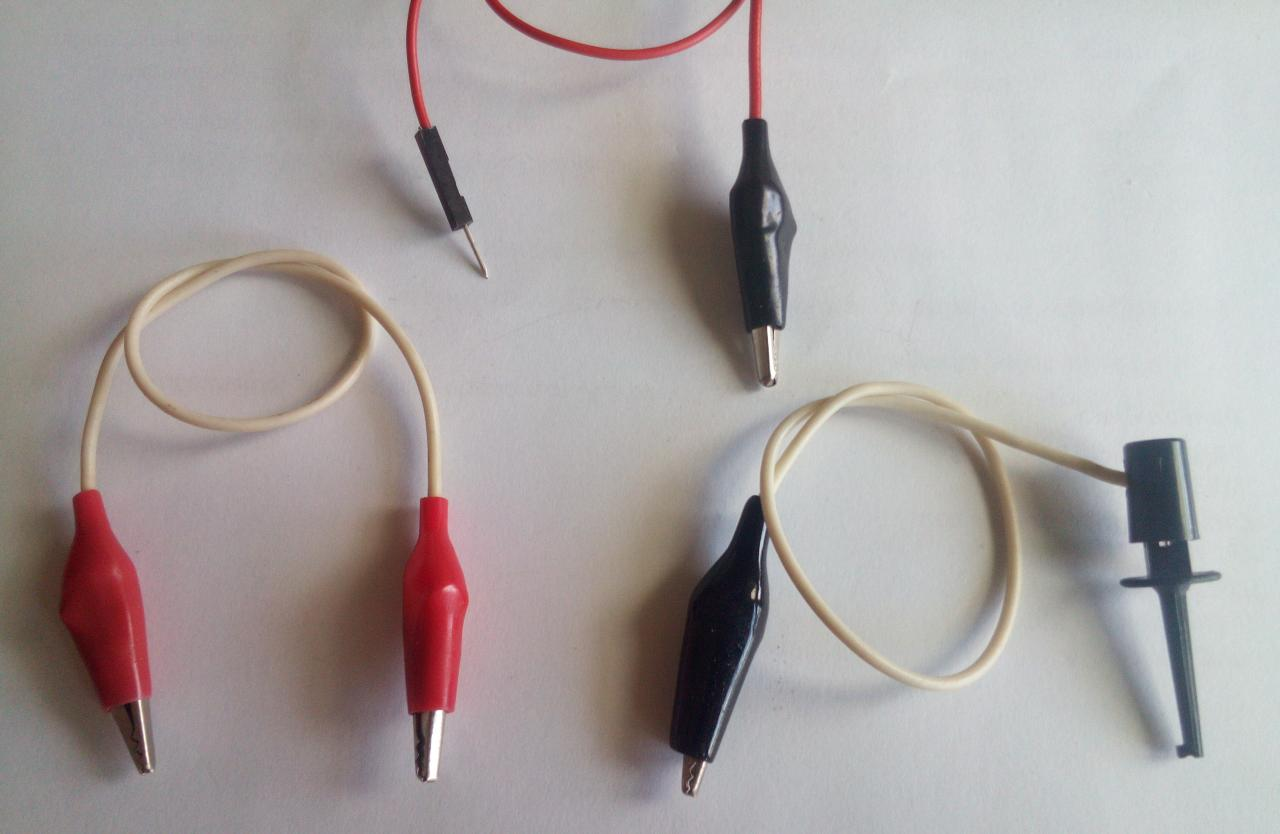
\includegraphics[height=5.3cm]{warsztat_elektroniczny/krokodylki}\footnotesize
		\\od lewej: przewód krokodylek - krokodylek (biało-czerwony), krokodylek - pin męski (czerwono-czarny), krokodylek - chwytak (biało-czarny)
	}
\hspace{\stretch{2}}
\vspace{12pt}

Koszt płytki prototypowej, zestawu kabelków i śrubokręta to około 20PLN.
